


\documentclass[a4paper,12pt,spanish]{article}

\usepackage[utf8]{inputenc}


\usepackage{blindtext}
%\usepackage{microtype}
\usepackage{amsfonts, amsmath, amsthm, amssymb}
%\usepackage{fancyhdr}
%\usepackage{index}
%\usepackage{multicol}    

%\usepackage{booktabs}

\usepackage[T1]{fontenc}
\usepackage[utf8]{inputenc}
\usepackage{graphicx}
\usepackage[spanish,es-tabla]{babel}
\usepackage{url}
\usepackage{enumitem}

\usepackage[unicode=true, pdfusetitle,
bookmarks=true,bookmarksnumbered=false,bookmarksopen=false,
breaklinks=true,pdfborder={0 0 1},backref=false,colorlinks=false]
{hyperref}

\usepackage{listings}
\usepackage{longtable}


\usepackage{siunitx} %para el sistema internacional
\usepackage[export]{adjustbox}
\usepackage{booktabs} 
\usepackage{subcaption}

\usepackage{float}


\newcommand{\address}[1]{
	\par {\raggedright #1
		\vspace{1.4em}
		\noindent\par}
}

\usepackage[table,xcdraw]{xcolor}


\pagenumbering{gobble}
\include{noNumberPage}
\pagenumbering{arabic}
\setcounter{page}{1}

%tutorial de tablas latex: https://manualdelatex.com/tutoriales/tablas

\usepackage{multirow}

% \usepackage[table,xcdraw]{xcolor}


%Inicio del documento (hasta que se cierre con \end{document}
\begin{document}
	
	
	\title{ Relación de dispersión de ondas de tensión superficial}
	
	%\author{Adrián Rivero Fernández}
	\date{}
	
	\maketitle
	
	%\vspace{\baselineskip}
	
	\section{Objetivos de la práctica}
	
	\begin{enumerate}
		\item Verificar la ley de Hagen-Poiseuille a partir de la experimentación con fluidos newtonianos que circulando a través de conductos capilares de diferentes diámetros.
		\item Caracterizar el régimen de circulación del fluido mediante el número de Reynolds.
		\item Determinar el coeficiente de rozamiento del conducto capilar.
	\end{enumerate}
	
	
	
	\section{Resumen teórico}
	
	A causa de la diferencia de presión entre los extremos de un tubo, se produce el flujo del fluido que contiene. Si registramos las velocidades volumetricas de flujo Q en función de la diferencia de presión $\mathit{\Delta }p$, vemos que la curva viene dada por las propiedades del fluido en cuestión y la geometría del tubo. El régimen del fluido se puede caracterizar por el número de Reynolds:
	\[ Re = \frac{\nu\rho D}{\mu}
	\]
	siendo $v$ la velocidad del flujo, $\rho$ la densidad, $\mu $ el coeficiente de viscosidad dinámica y $D$ una longitud característica del sistema, que para un fluido circulando por un tubo se considera su diámetro. 
	
	Un bajo número de Reynolds, aproximadamente por debajo de 2000, se considera régimen laminar. En este régimen los fluidos presentan una elevada viscosidad y circulan a baja velocidad, o circulan por tuberías de pequeña sección. 
	
	Un alto número de Reynolds, por encima de 3000, se llama régimen turbulento, y los fluidos tienen baja viscosidad y alta velocidad o avanzan por tuberías de gran sección. Para un fluido se puede identificar el cambio de régimen laminar a turbulento en la gráfica de $Q$ frente a $\mathit{\Delta}p$. El valor del número de Reynolds en ese punto es el llamado Reynolds crítico.\\
	
	
	Por la ley de Hagen-Poiseuille, podemos obtener la velocidad promedio como
	
	\[U = \frac{Q}{\pi R^2} = \frac{R^2 \mathit{\Delta} p}{8\mu l}\]
	
	Con esta velocidad promedio $U$ se puede calcular el número de Reynolds, $Re$, usando $U$ como velocidad característica $\nu$ y el diámetro $d$ como longitud característica $D$.
	
	\[Re = \frac{\nu \rho D}{\mu}= \frac{U \rho d}{\mu}\] 
	
	\vspace{\baselineskip}
	
	El coeficiente de rozamiento $\lambda$, factor de fricción o coeficiente de resistencia de Darcy-Weisbach se usa para evaluar las pérdidas viscosas. Podemos obtener $\lambda$ con la expresión
	\[\lambda = \frac{d}{L} \cdot \frac{\rho g h_f}{\frac{1}{2} \rho U^2} = \frac{d}{L} \cdot \frac{\mathit{\Delta}p}{\frac{1}{2} \rho U^2}\]
	
	Para tubos horizontales de sección circular y régimen laminar, el factor de fricción es 
	\[\lambda = \frac{64}{Re}\]
	
	El coeficiente de rozamiento $\lambda$ frente a $Re$ para distintos valores de $h/d$ para una forma de conducto fija se representa en los llamados diagramas de Moody, que generalmente están en escala log-log.
	
	
	
	\section{Procedimiento experimental}
	
	\begin{enumerate}
		\item Insertamos el capilar de vidrio con el diámetro a estudiar en el tubo vertical y lo sujetamos en posición horizontal con una pinza.
		\item Nivel el tubo vertical y el capilar horizontal.
		\item Conectamos la manguera al grifo y rellenar el tubo vertical de agua hasta aproximadamente 40 cm de altura.
		\item Medimos la temperatura de este agua en el interior del tubo y determinamos el valor de la viscosidad dinámica
		\item  Con el agua fluyendo por el tubo capilar, regulamos el caudal del grifo llenando el tubo vertical para que el nivel del agua se mantenga constante en una misma altura, de modo que el caudal de salida por el capilar coincide con el caudal de entrada del grifo.
		\item Recogemos en un vaso de precipitados el agua que se vierte del tubo capilar en un intervalo de 10s para diferentes alturas del nivel del agua.
		\item Determinamos el diámetro del tubo capilar según la cantidad máxima de masa de agua que puede llegar a contener. Para ello rellenamos el tubo con agua, lo vertemos en un vaso de precipitados, que posteriormente pesamos.
	\end{enumerate}
	
	
\begin{figure}[H]
	\centering
	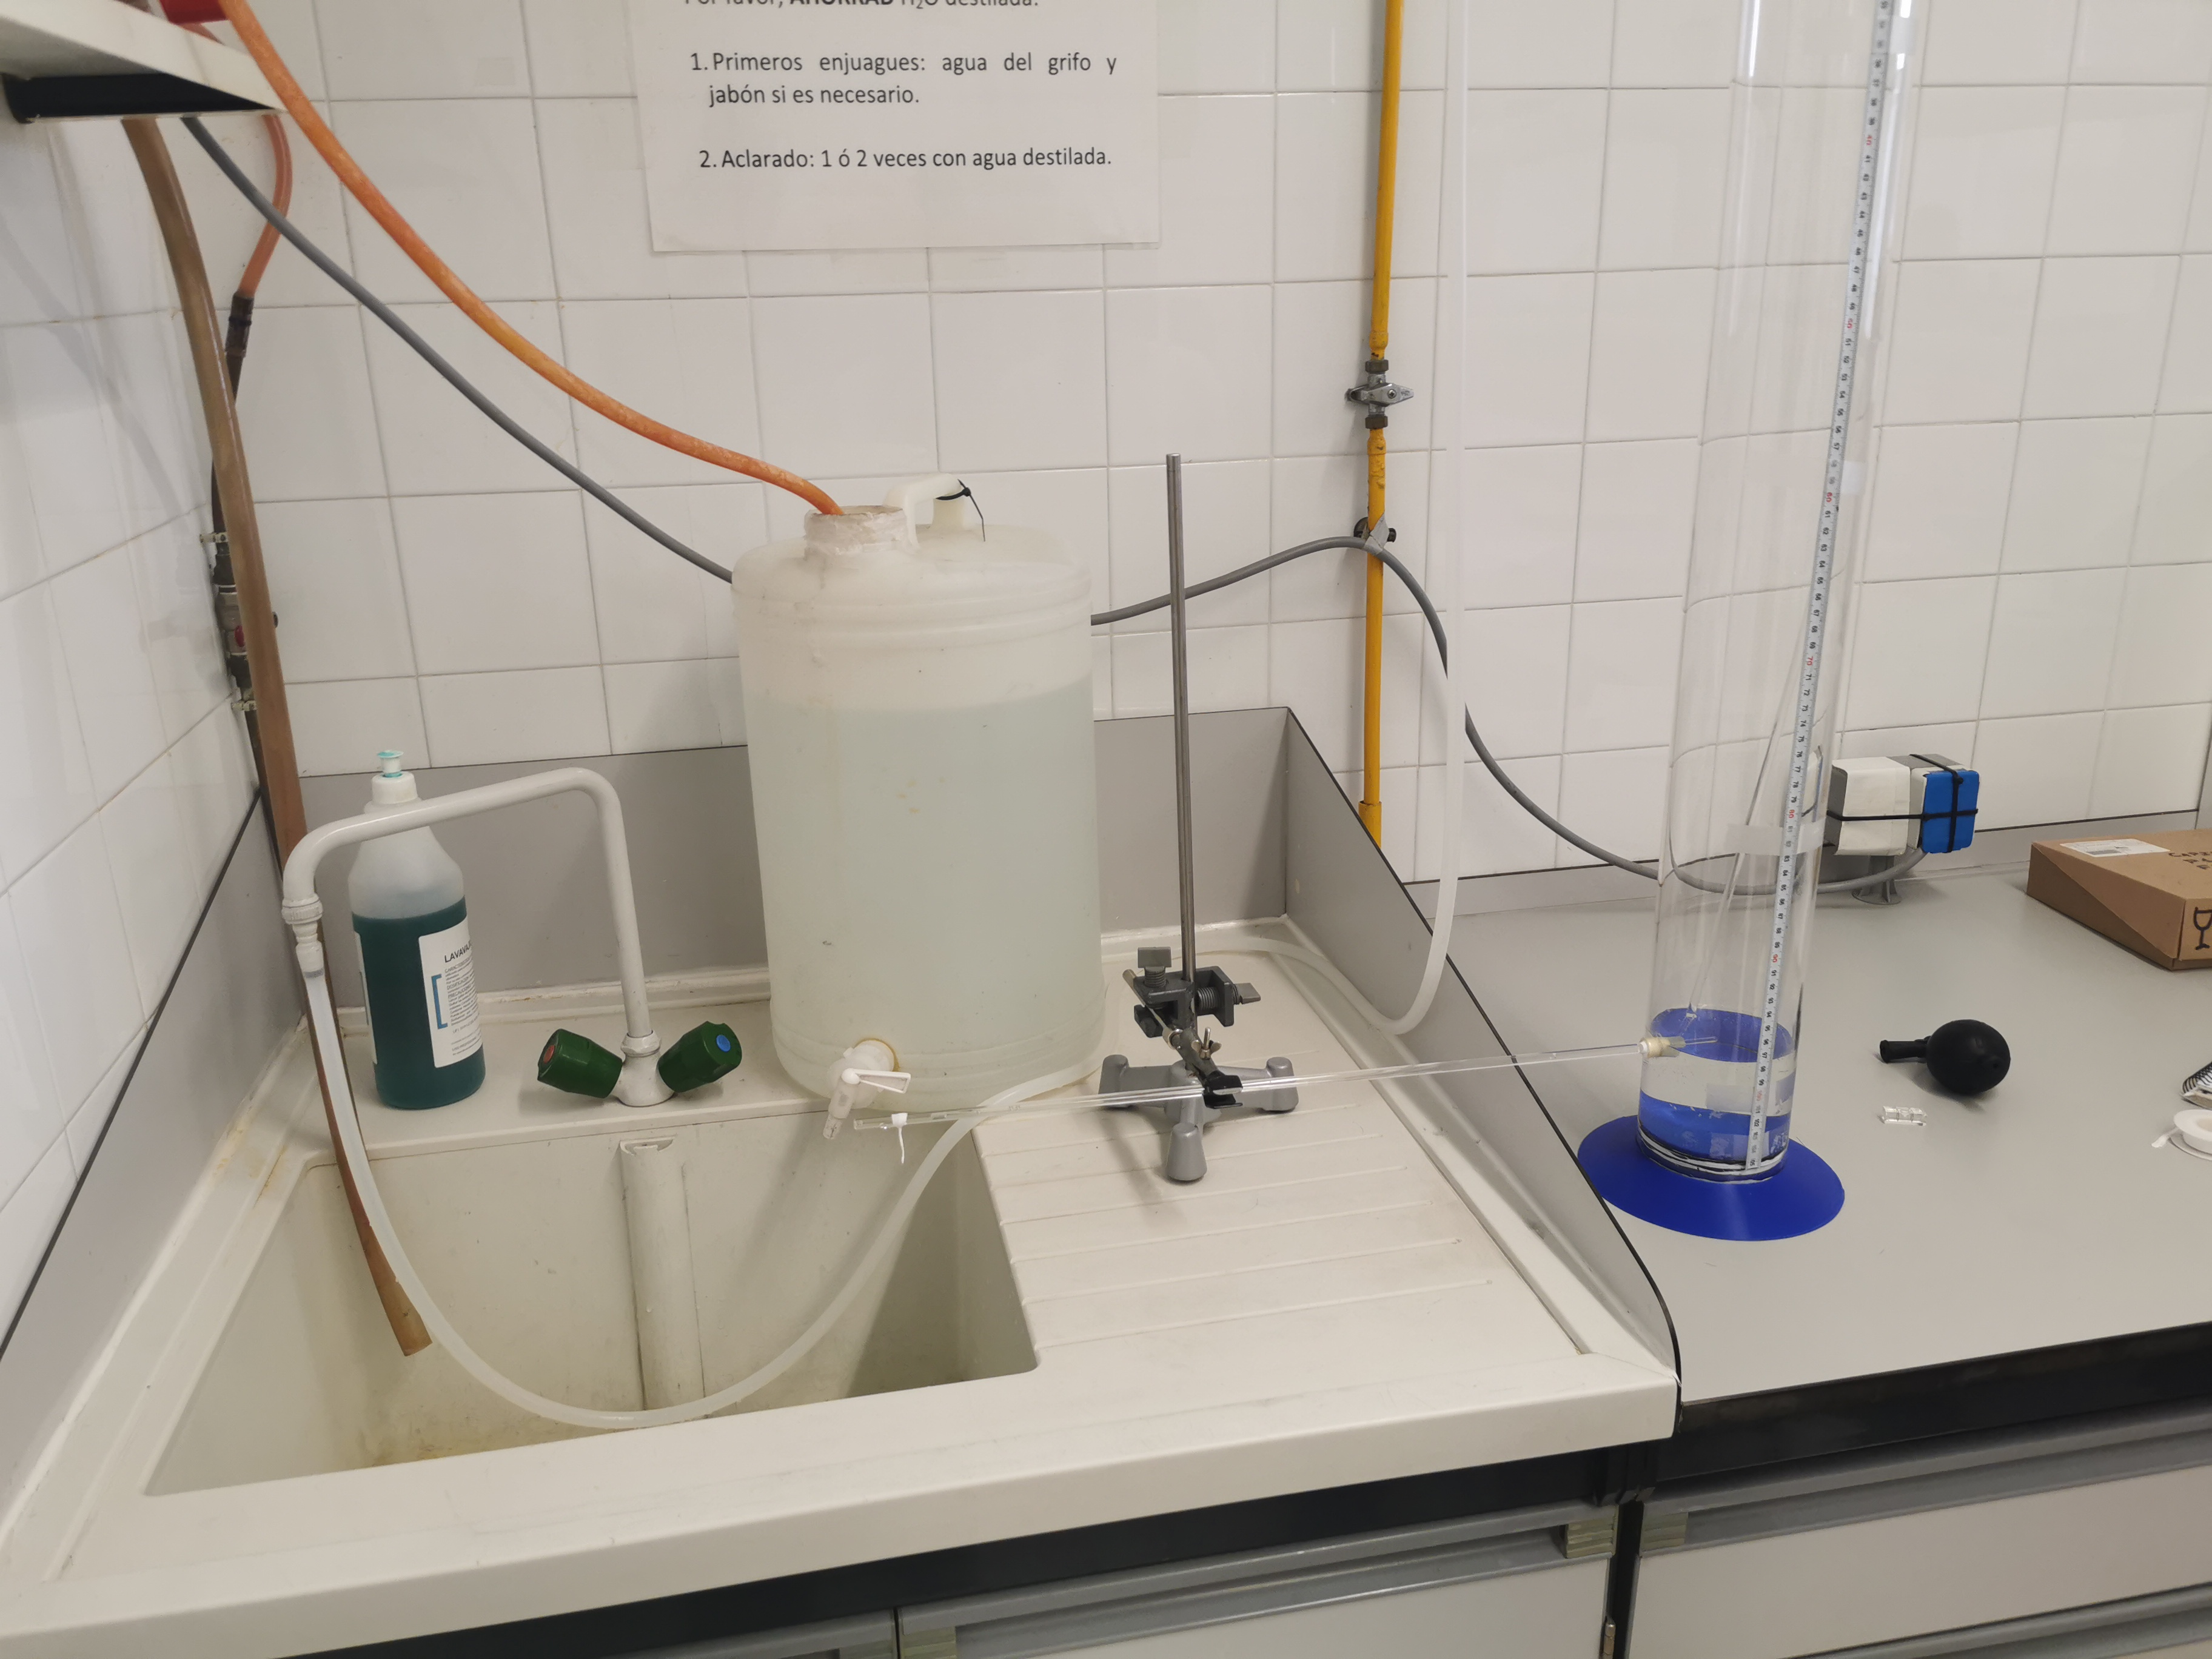
\includegraphics[width=0.7\linewidth]{../IMG_20240307_124615}
	\caption{Dispositivo experimental: tubo vertical conectado a tubo de menor sección horizontal, con una manguera podemos introducir más agua en el tubo}
	\label{fig:img20240307124615}
\end{figure}
	
	\section{Tablas de medidas}
	
	
	El tubo horizontal tiene una regla graduada en sentido descendente que nos permitirá ajustar la altura de agua a correctos intervalos, estas distancias son la medida $D$. El valor real de la altura, $h$, lo obtenemos restando $D$ a la altura real en el tubo a la que situamos el origen de la regla, $98\pm 1 $ cm.\\

	La medida de masa del vaso con agua es $m_{tot}$, que restando la masa del vaso vacío nos da la masa de agua
	\[ m_{tot} = m_{agua} + m_{vaso}
	\]
	\[ m_{vaso} = 182,86 \pm 0,01 \si{g}
	\]
	
	Obtenemos el caudal y su error calculado por propagación de errores
	\[ Q = \frac{m_{agua}}{\rho t}
	\]
	\[\Delta Q = \frac{1}{\rho t} \Delta m+ \frac{m}{t\rho^2}\Delta \rho + \frac{m}{\rho t^2}\Delta t
	\]
	
	La diferencia de presión con su error
	\[ \mathit{\Delta} p = \rho g h
	\]
	\[ \Delta (\mathit{\Delta} p) = g h \Delta \rho + \rho h \Delta g + \rho g \Delta h 
	\]
	
	
	\vspace{\baselineskip}
	
	Otras medidas relevantes sobre nuestro sistema experimental:
	
	\begin{itemize}
		\item Error en medida de tiempo: $\Delta t = \pm 0,5 \si{s}$
		\item Densidad del agua: $\rho = 0,998\pm 0,001 \si{g/cm^3 }$
		\item Gravedad: $g = 981\pm 1 \si{cm/s^2}$
	\end{itemize}
	
	\vspace{\baselineskip}
	
	
	
	
	\begin{table}[H]
		\centering
		\begin{tabular}{cccccccc}
			\hline
			\multicolumn{1}{|c|}{D (cm)} & \multicolumn{1}{c|}{h (cm)} & \multicolumn{1}{c|}{$m_{tot}$ (g)} & \multicolumn{1}{c|}{$m_{agua}$  (g)} & \multicolumn{1}{c|}{$Q$ (cm$^3$/s)} & \multicolumn{1}{c|}{$\Delta Q$} & \multicolumn{1}{c|}{$\mathit{\Delta} p$(cm$^{-1}$s$^{-2}$g)} & \multicolumn{1}{c|}{$\Delta \mathit{\Delta}p$} \\ \hline\hline
			\multicolumn{1}{|c|}{30,0} & \multicolumn{1}{c|}{68,0} & \multicolumn{1}{c|}{269,12} & \multicolumn{1}{c|}{86,26} & \multicolumn{1}{c|}{8,6} & \multicolumn{1}{c|}{0,4} & \multicolumn{1}{c|}{66500} & \multicolumn{1}{c|}{300} \\ \hline
			\multicolumn{1}{|c|}{35,4} & \multicolumn{1}{c|}{62,6} & \multicolumn{1}{c|}{262,86} & \multicolumn{1}{c|}{80,00} & \multicolumn{1}{c|}{8,0} & \multicolumn{1}{c|}{0,4} & \multicolumn{1}{c|}{61300} & \multicolumn{1}{c|}{300} \\ \hline
			\multicolumn{1}{|c|}{40,4} & \multicolumn{1}{c|}{57,6} & \multicolumn{1}{c|}{261,28} & \multicolumn{1}{c|}{78,42} & \multicolumn{1}{c|}{7,8} & \multicolumn{1}{c|}{0,4} & \multicolumn{1}{c|}{56400} & \multicolumn{1}{c|}{300} \\ \hline
			\multicolumn{1}{|c|}{45,0} & \multicolumn{1}{c|}{53,0} & \multicolumn{1}{c|}{257,62} & \multicolumn{1}{c|}{74,76} & \multicolumn{1}{c|}{7,5} & \multicolumn{1}{c|}{0,4} & \multicolumn{1}{c|}{51900} & \multicolumn{1}{c|}{300} \\ \hline
			\multicolumn{1}{|c|}{50,0} & \multicolumn{1}{c|}{48,0} & \multicolumn{1}{c|}{257,03} & \multicolumn{1}{c|}{74,17} & \multicolumn{1}{c|}{7,4} & \multicolumn{1}{c|}{0,4} & \multicolumn{1}{c|}{45000} & \multicolumn{1}{c|}{300} \\ \hline
			\multicolumn{1}{|c|}{55,2} & \multicolumn{1}{c|}{42,8} & \multicolumn{1}{c|}{251,52} & \multicolumn{1}{c|}{68,66} & \multicolumn{1}{c|}{6,9} & \multicolumn{1}{c|}{0,4} & \multicolumn{1}{c|}{51900} & \multicolumn{1}{c|}{300} \\ \hline
			\multicolumn{1}{|c|}{60,2} & \multicolumn{1}{c|}{37,8} & \multicolumn{1}{c|}{250,47} & \multicolumn{1}{c|}{67,61} & \multicolumn{1}{c|}{6,8} & \multicolumn{1}{c|}{0,3} & \multicolumn{1}{c|}{37000} & \multicolumn{1}{c|}{300} \\ \hline
			\multicolumn{1}{|c|}{65,2} & \multicolumn{1}{c|}{32,8} & \multicolumn{1}{c|}{248,30} & \multicolumn{1}{c|}{65,44} & \multicolumn{1}{c|}{6,5} & \multicolumn{1}{c|}{0,3} & \multicolumn{1}{c|}{32100} & \multicolumn{1}{c|}{300} \\ \hline
			\multicolumn{1}{|c|}{70,2} & \multicolumn{1}{c|}{27,8} & \multicolumn{1}{c|}{243,77} & \multicolumn{1}{c|}{60,91} & \multicolumn{1}{c|}{6,1} & \multicolumn{1}{c|}{0,3} & \multicolumn{1}{c|}{27200} & \multicolumn{1}{c|}{300} \\ \hline
			\multicolumn{1}{|c|}{75,0} & \multicolumn{1}{c|}{23,0} & \multicolumn{1}{c|}{235,59} & \multicolumn{1}{c|}{52,73} & \multicolumn{1}{c|}{5,3} & \multicolumn{1}{c|}{0,3} & \multicolumn{1}{c|}{22500} & \multicolumn{1}{c|}{200} \\ \hline
			\multicolumn{1}{|c|}{80,0} & \multicolumn{1}{c|}{18,0} & \multicolumn{1}{c|}{225,24} & \multicolumn{1}{c|}{42,38} & \multicolumn{1}{c|}{4,2} & \multicolumn{1}{c|}{0,2} & \multicolumn{1}{c|}{17600} & \multicolumn{1}{c|}{200} \\ \hline
			\multicolumn{1}{|c|}{82,0} & \multicolumn{1}{c|}{16,0} & \multicolumn{1}{c|}{222,14} & \multicolumn{1}{c|}{39,28} & \multicolumn{1}{c|}{3,9} & \multicolumn{1}{c|}{0,2} & \multicolumn{1}{c|}{16000} & \multicolumn{1}{c|}{200} \\ \hline
			\multicolumn{1}{|c|}{84,0} & \multicolumn{1}{c|}{14,0} & \multicolumn{1}{c|}{217,59} & \multicolumn{1}{c|}{34,73} & \multicolumn{1}{c|}{3,5} & \multicolumn{1}{c|}{0,2} & \multicolumn{1}{c|}{13700} & \multicolumn{1}{c|}{200} \\ \hline
			\multicolumn{1}{|c|}{86,0} & \multicolumn{1}{c|}{12,0} & \multicolumn{1}{c|}{214,03} & \multicolumn{1}{c|}{31,17} & \multicolumn{1}{c|}{3,1} & \multicolumn{1}{c|}{0,2} & \multicolumn{1}{c|}{11700} & \multicolumn{1}{c|}{200} \\ \hline
			\multicolumn{1}{|c|}{88,0} & \multicolumn{1}{c|}{10,0} & \multicolumn{1}{c|}{209,26} & \multicolumn{1}{c|}{26,40} & \multicolumn{1}{c|}{2,64} & \multicolumn{1}{c|}{0,14} & \multicolumn{1}{c|}{9800} & \multicolumn{1}{c|}{200} \\ \hline
			\multicolumn{1}{|c|}{90,0} & \multicolumn{1}{c|}{8,0} & \multicolumn{1}{c|}{204,77} & \multicolumn{1}{c|}{21,91} & \multicolumn{1}{c|}{2,19} & \multicolumn{1}{c|}{0,11} & \multicolumn{1}{c|}{7800} & \multicolumn{1}{c|}{200} \\ \hline
			\multicolumn{1}{|c|}{91,0} & \multicolumn{1}{c|}{7,0} & \multicolumn{1}{c|}{202,50} & \multicolumn{1}{c|}{19,64} & \multicolumn{1}{c|}{1,96} & \multicolumn{1}{c|}{0,10} & \multicolumn{1}{c|}{6900} & \multicolumn{1}{c|}{200} \\ \hline
			\multicolumn{1}{|c|}{92,0} & \multicolumn{1}{c|}{6,0} & \multicolumn{1}{c|}{199,51} & \multicolumn{1}{c|}{16,65} & \multicolumn{1}{c|}{1,67} & \multicolumn{1}{c|}{0,09} & \multicolumn{1}{c|}{5900} & \multicolumn{1}{c|}{200} \\ \hline
			\multicolumn{1}{|c|}{93,3} & \multicolumn{1}{c|}{4,7} & \multicolumn{1}{c|}{194,69} & \multicolumn{1}{c|}{11,83} & \multicolumn{1}{c|}{1,18} & \multicolumn{1}{c|}{0,06} & \multicolumn{1}{c|}{4600} & \multicolumn{1}{c|}{200} \\ \hline
			\multicolumn{1}{|c|}{93,9} & \multicolumn{1}{c|}{4,1} & \multicolumn{1}{c|}{192,73} & \multicolumn{1}{c|}{9,87} & \multicolumn{1}{c|}{0,99} & \multicolumn{1}{c|}{0,05} & \multicolumn{1}{c|}{4000} & \multicolumn{1}{c|}{200} \\ \hline
			\multicolumn{1}{|c|}{94,6} & \multicolumn{1}{c|}{3,4} & \multicolumn{1}{c|}{190,44} & \multicolumn{1}{c|}{7,58} & \multicolumn{1}{c|}{0,76} & \multicolumn{1}{c|}{0,04} & \multicolumn{1}{c|}{3300} & \multicolumn{1}{c|}{200} \\ \hline
			\multicolumn{1}{|c|}{95,0} & \multicolumn{1}{c|}{3,0} & \multicolumn{1}{c|}{188,95} & \multicolumn{1}{c|}{6,09} & \multicolumn{1}{c|}{0,61} & \multicolumn{1}{c|}{0,03} & \multicolumn{1}{c|}{2900} & \multicolumn{1}{c|}{200} \\ \hline
			\multicolumn{1}{|c|}{95,7} & \multicolumn{1}{c|}{2,3} & \multicolumn{1}{c|}{187,20} & \multicolumn{1}{c|}{4,34} & \multicolumn{1}{c|}{0,43} & \multicolumn{1}{c|}{0,02} & \multicolumn{1}{c|}{2300} & \multicolumn{1}{c|}{200} \\ \hline
			\multicolumn{1}{|c|}{96,6} & \multicolumn{1}{c|}{1,4} & \multicolumn{1}{c|}{185,01} & \multicolumn{1}{c|}{0,215} & \multicolumn{1}{c|}{0,013} & \multicolumn{1}{c|}{0,01} & \multicolumn{1}{c|}{1400} & \multicolumn{1}{c|}{200} \\ \hline
			\multicolumn{1}{l}{} & \multicolumn{1}{l}{} & \multicolumn{1}{l}{} & \multicolumn{1}{l}{} & \multicolumn{1}{l}{} & \multicolumn{1}{l}{} & \multicolumn{1}{l}{} & \multicolumn{1}{l}{} \\ \cline{1-4}
			\multicolumn{1}{|c|}{$\Delta D   $} & \multicolumn{1}{c|}{$\Delta h  $} & \multicolumn{1}{c|}{$\Delta m_{tot}  $} & \multicolumn{1}{c|}{$\Delta m_{agua} $} &  &  &  &  \\ \cline{1-4}
			\multicolumn{1}{|c|}{$\pm 0,1$} & \multicolumn{1}{c|}{$\pm0,2$} & \multicolumn{1}{c|}{$\pm0,01$} & \multicolumn{1}{c|}{$\pm0,02$} &  &  &  &  \\ \cline{1-4}
		\end{tabular}
		\caption{Caudal y diferencia de presión en función de la masa de agua expulsada a distintas alturas}
		\label{tab:QDeltap}
	\end{table}
	
	\vspace{\baselineskip}
	
	
	Para obtener las medidas del capilar, lo llenamos de agua, lo pesamos varias veces y calculamos la media, para reducir el error, que debemos calcular según su desviación típica:
	
	
	\begin{table}[H]
		\centering
		\begin{tabular}{c|c|c|}
			\cline{2-3}
			& Valor & Error \\ \hline
			\multicolumn{1}{|c|}{Medida 1} & 45,67 & 0,01 \\ \hline
			\multicolumn{1}{|c|}{Medida 2} & 45,60 & 0,01 \\ \hline
			\multicolumn{1}{|c|}{Medida 3} & 45,66 & 0,01 \\ \hline\hline								
			\multicolumn{1}{|c|}{Media} & 45,64 & 0,02 \\ \hline
		\end{tabular}
	\caption{Media de las medidas de masa del capilar con agua}
	\end{table}
	
	
	De modo que la masa del capilar con agua es 
	\[ m_{total} = 45,64 \pm 0,02 \si{g} \]
	
	Ahora, pesamos el capilar sin agua, y restándolo al valor anterior obtenemos la masa (y por tanto el volumen) del agua en el interior del capilar.
	

	\[m_{capilar} = 41,45\pm 0,01 \si{g}\]
	\[ m_{agua} = 4,19 \pm 0,03 \si{g}\]
	\[V_{agua} = \frac{m_{agua}}{\rho} = 4,20 \pm 0,03 \si{cm^3}\]
	
	Donde el error $\Delta m_{agua}$ ha sido propagado
	\[ \Delta m_{agua} = \left|\frac{\partial m_{agua}}{\partial m_{total}}\right|\Delta m_{total} + \left|\frac{\partial m_{agua}}{\partial m_{capilar}}\right|\Delta m_{capilar}
	\]
	
	\vspace{\baselineskip}
	
	La longitud del capilar ha sido medida como:
	\[l = 60\pm 1\si{cm} \]
	
	
	
	
	\vspace{\baselineskip}
	
	
	
	
	
	Ahora para obtener el radio, partimos del volumen
	\[V = \pi R^2 \cdot l \longrightarrow R = \sqrt{\frac{V}{\pi l}}\]
	\[ \Delta R = \frac{1}{2\sqrt{\pi l V}} \Delta V + \frac{1}{2}\sqrt{\frac{V}{\pi l^3}}\Delta l
	\]
	\[ R = 0,149 \pm 0,002 \si{cm}
	\]
	Y por tanto su diámetro
	\[ d = 0,299\pm 0,004 \si{cm}
	\]
	
	%oh dios mio propagar esto va a ser horrible
	
	
	
	
	\iffalse
	
	\begin{itemize}
		\item 
	\end{itemize}
	
	
	
	\item masa capilar con agua: $45,64\pm 0,01 \si{g}$
	\item masa capilar sin agua: $41,45\pm 0,01 \si{g}$
	\item longitud del capilar: $l = 60\pm 1\si{cm}$
	\item masa agua en capilar	4,1933333333333    % mucho de esto es dependiente, por lo que hay que calcularlo, o sea QUITAR DE AQUI LAS QUE NO SEAN DIRECTAS!!!!!
	\item volumen de agua en capilar (cm3)	4,1933333333333
	\item radio capilar	0,149152017310305
	\item diametro (cm)	0,298304034620611
	
	masa capilar con agua	45,67
	45,6
	45,66
	media	45,6433333333333
	\fi
	
	
	
	\section{Gráficas}
	
	
	
	\begin{figure}[H]
		\centering
		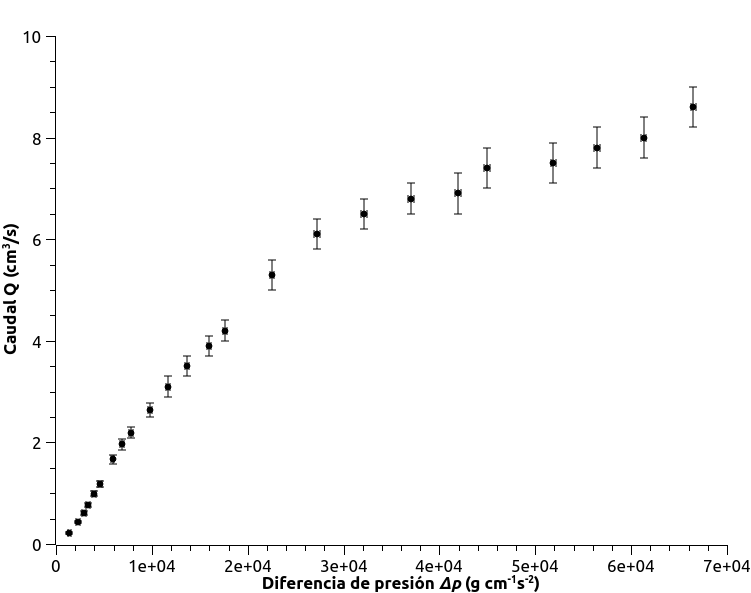
\includegraphics[width=0.9\linewidth]{graficas/caudal_presion}
		\caption{Representación del caudal frente diferencia de presión para distintas alturas del agua}
		\label{fig:caudalpresion}
	\end{figure}
	
	
	\begin{longtable}[c]{|c|c|c|c|}
		
		
			\hline
			$\mathit{\Delta}p$ [X]& $\Delta\mathit{\Delta}p$ [err X] & $Q$ [Y]& $\Delta Q$ [err Y]\\ \hline\hline
			\endfirsthead
			\endhead
			66500 & 300 & 8,6 & 0,4 \\ \hline
			61300 & 300 & 8 & 0,4 \\ \hline
			56400 & 300 & 7,8 & 0,4 \\ \hline
			51900 & 300 & 7,5 & 0,4 \\ \hline
			45000 & 300 & 7,4 & 0,4 \\ \hline
			41900 & 300 & 6,9 & 0,4 \\ \hline
			37000 & 300 & 6,8 & 0,3 \\ \hline
			32100 & 300 & 6,5 & 0,3 \\ \hline
			27200 & 300 & 6,1 & 0,3 \\ \hline
			22500 & 200 & 5,3 & 0,3 \\ \hline
			17600 & 200 & 4,2 & 0,2 \\ \hline
			16000 & 200 & 3,9 & 0,2 \\ \hline
			13700 & 200 & 3,5 & 0,2 \\ \hline
			11700 & 200 & 3,1 & 0,2 \\ \hline
			9800 & 200 & 2,64 & 0,14 \\ \hline
			7800 & 200 & 2,19 & 0,11 \\ \hline
			6900 & 200 & 1,96 & 0,10 \\ \hline
			5900 & 200 & 1,67 & 0,09 \\ \hline
			4600 & 200 & 1,18 & 0,06 \\ \hline
			4000 & 200 & 0,99 & 0,05 \\ \hline
			3300 & 200 & 0,76 & 0,04 \\ \hline
			2900 & 200 & 0,61 & 0,03 \\ \hline
			2300 & 200 & 0,43 & 0,02 \\ \hline
			1400 & 200 & 0,215 & 0,013 \\ \hline
		
		\caption{Tabla de datos de la Figura \ref{fig:caudalpresion}}
	\end{longtable}
	
	
	\iffalse
	\begin{table}[H]
		\centering
		\begin{tabular}{|c|c|c|c|}
			\hline
			$\mathit{\Delta}p$ [X]& $\Delta\mathit{\Delta}p$ [err X] & $Q$ [Y]& $\Delta Q$ [err Y]\\ \hline\hline
			66500 & 300 & 8,6 & 0,4 \\ \hline
			61300 & 300 & 8 & 0,4 \\ \hline
			56400 & 300 & 7,8 & 0,4 \\ \hline
			51900 & 300 & 7,5 & 0,4 \\ \hline
			45000 & 300 & 7,4 & 0,4 \\ \hline
			41900 & 300 & 6,9 & 0,4 \\ \hline
			37000 & 300 & 6,8 & 0,3 \\ \hline
			32100 & 300 & 6,5 & 0,3 \\ \hline
			27200 & 300 & 6,1 & 0,3 \\ \hline
			22500 & 200 & 5,3 & 0,3 \\ \hline
			17600 & 200 & 4,2 & 0,2 \\ \hline
			16000 & 200 & 3,9 & 0,2 \\ \hline
			13700 & 200 & 3,5 & 0,2 \\ \hline
			11700 & 200 & 3,1 & 0,2 \\ \hline
			9800 & 200 & 2,64 & 0,14 \\ \hline
			7800 & 200 & 2,19 & 0,11 \\ \hline
			6900 & 200 & 1,96 & 0,10 \\ \hline
			5900 & 200 & 1,67 & 0,09 \\ \hline
			4600 & 200 & 1,18 & 0,06 \\ \hline
			4000 & 200 & 0,99 & 0,05 \\ \hline
			3300 & 200 & 0,76 & 0,04 \\ \hline
			2900 & 200 & 0,61 & 0,03 \\ \hline
			2300 & 200 & 0,43 & 0,02 \\ \hline
			1400 & 200 & 0,215 & 0,013 \\ \hline
		\end{tabular}
		\caption{Tabla de datos de la Figura \ref{fig:caudalpresion}}
	\end{table}
	\fi
	
	\begin{figure}[H]
		\centering
		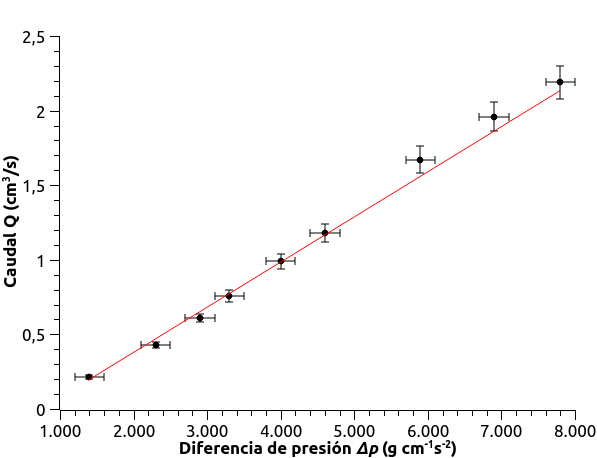
\includegraphics[width=0.7\linewidth]{graficas/caudal_laminar}
		\caption{Región laminar de la Figura \ref{fig:caudalpresion}}
		\label{fig:caudallaminar}
	\end{figure}
	
	\begin{table}[H]
		\centering
		\begin{tabular}{|c|c|c|c|}
			\hline
			$\mathit{\Delta}p$ [X]& $\Delta\mathit{\Delta}p$ [err X] & $Q$ [Y]& $\Delta Q$ [err Y]\\ \hline\hline
			7800 & 200 & 2,19 & 0,11 \\ \hline
			6900 & 200 & 1,96 & 0,1 \\ \hline
			5900 & 200 & 1,67 & 0,09 \\ \hline
			4600 & 200 & 1,18 & 0,06 \\ \hline
			4000 & 200 & 0,99 & 0,05 \\ \hline
			3300 & 200 & 0,76 & 0,04 \\ \hline
			2900 & 200 & 0,61 & 0,03 \\ \hline
			2300 & 200 & 0,43 & 0,02 \\ \hline
			1400 & 200 & 0,215 & 0,013 \\ \hline
		\end{tabular}
		\caption{Tabla de datos de la Figura \ref{fig:caudallaminar}}
	\end{table}
	
	
	
	
	
	\iffalse
	B (y-intercección) = -0,227877457028667 +/- 0,0204241529800304
	A (pendiente) = 0,000302759774035129 +/- 8,30618954225738e-06
	--------------------------------------------------------------------------------------
	Chi^2 = 10,5663151320189
	R^2 = 0,992109752840265
	---------------------------------------------------------------------
	\fi
	
	El ajuste de mínimos cuadrados de la Figura \ref{fig:caudallaminar} es
	\[ Q = A\cdot \mathit{\Delta }p + B
	\]
	\[ A = (3,03 \pm 0,08) \cdot 10^{-4} \si{cm^4 s / g}   % +/- 8,30618954225738e-06 %0,083
	\]
	\[B = (-0,28 \pm 0,02) \si{g\cdot cm^{-1} s^{-2}}   %-0,227877457028667 +/- 0,0204241529800304
	\]
	
	Con una coeficiente de correlación
	\[ R^2 = 0,9921
	\] 
	
	
	
	
	
	\section{Discusión de resultados} 
	
	\subsection*{Gráfica Caudal-Presión}
	
	En la Figura \ref{fig:caudalpresion} vemos como el caudal se incrementa a mayor diferencia de presión, de modo que la curva es ascendente. Para valores pequeños, para valores $\mathit{\Delta }p \leq 7800$, la figura toma una forma lineal.\\
	
	En la Figura \ref{fig:caudallaminar} está representada esa sección lineal, correspondiente a la región de flujo laminar.
	
	\subsection*{Viscosidad dinámica}
	
	
	Con el ajuste por mínimos cuadrados en la Figura \ref{fig:caudallaminar} y la expresión de la ley de Hagen-Poiseuille, podemos despejar la viscosidad dinámica
	
	
	\[U = \frac{Q}{\pi R^2} = \frac{R^2 \mathit{\Delta} p}{8\mu l} \longrightarrow \mu = \frac{R^4\pi \mathit{\Delta p}}{Q 8 l}
	\] 
	La pendiente de la recta de ajuste
	
	\[A = \frac{Q}{\mathit{\Delta}p} = (3,03 \pm 0,08) \cdot 10^{-4} \si{cm^4 s / g} \]
	
	De modo que podemos sustituir
	\[ \mu = \frac{R^4\pi }{A 8 l}
	\]
	\[ \Delta \mu = \left| \frac{4R^3\pi}{8A\cdot l} 
	\right| \Delta R + \left| -\frac{R^4 \pi }{8A \cdot l^2}
	  \right| \Delta l + \left| -\frac{R^4 \pi}{8 A^2 \cdot l}
	  \right| \Delta A
	\]
	
	Obteniendo finalmente
	
	\[  \mu = 0,011 \pm 0,001 \si{{g}/(s\cdot cm)}
	\]
	
	En la literatura, el valor de la viscosidad dinámica del agua a 20ºC es 
	\[ \mu_{lit} = 0,001 \si{[Pa\cdot s]} = 0,001 \si{[kg\cdot m^{-1}\cdot s^{-1}]} =
	\]
	\[  = 0,01 [\si{g\cdot cm^{-1}\cdot s^{-1}}]
	\]
	
	Este valor de viscosidad dinámica encaja perfectamente con el que hemos obtenido, ambos se encuentran en el margen de error del otro.
	
	
	
	\subsection*{Número de Reynolds}
	
	Como vimos 
	\[Re = \frac{\nu \rho D}{\mu}= \frac{U \rho d}{\mu}\] 
	Mientras el error
	\[ \Delta Re = \left|  \frac{\rho d}{\mu}\
	\right| \Delta U + \left| \frac{U  d}{\mu}\
	\right| \Delta \rho + \left| \frac{U \rho }{\mu}\
	\right| \Delta d + \left| -\frac{U \rho d}{\mu^2}\
	\right| \Delta \mu
	\]
	
	\iffalse
	\subsection*{Velocidad promedio}
	
	\[U = \frac{Q}{\pi R^2} \]
	\fi
	
	Tendremos que obtener el $Re$ para cada caudal $Q$ de los obtenidos en la Tabla \ref{tab:QDeltap}, calculando antes la velocidad promedio:
	\[ U = \frac{Q}{\pi R^2}
	\]
	\[ \Delta U = \left| \frac{1}{\pi R^2}
	\right|\Delta Q + \left| -2\frac{Q}{\pi R^3}
	\right| \Delta R
	\]
	
	\subsection*{Factor de fricción}
	
	\[\lambda = \frac{d}{L} \cdot \frac{\rho g h_f}{\frac{1}{2} \rho U^2} = \frac{d}{L} \cdot \frac{\mathit{\Delta}p}{\frac{1}{2} \rho U^2}\]

	\[\lambda = \frac{64}{Re}\]

	
	
	\section{Conclusiones}
	
	
	
	


\end{document}